\begin{center}
\emph{Enumerating permutations is sometimes hard and usually tedious. Packing permutations is often hard and always tedious.}
\end{center}
\begin{flushright}
  \vspace{-15pt}
  --- folklore
  \vspace{20pt}
\end{flushright}



This entire thesis is concerned with only one kind of object --- \emph{permutations}. We treat permutations as patterns or words that use every letter in the alphabet exactly once, the alphabet being $[n] = \{1,\ldots,n\}$. In fact, we study permutation classes rather than permutations themselves. These are collections of permutations closed under taking subpermutations. There are several natural approaches to studying permutation classes. Let $\C$ be a permutation class. Then one can enquire about the properties of a what a typical object from $\C$ ``looks'' like? Alternatively, one could be interested in how many permutations of each length are there in $\C$? Yet another different approach would be to ask questions such as what is the maximum number of inversions that a permutation in $\C$ can have? While all three are interesting directions of study, we focus on questions of the second and third kinds only.

The enumerative approach to permutation classes has been quite dominant in the permutation patterns community. There are several works that survey this area chronologically and systematically. We point to the chapter \emph{Permutation Classes} by Vatter~\cite{vatterhandbook} in the Handbook of Enumerative Combinatorics. For further book material, refer to the references therein. On the other hand, additional surveys of the field can be found in the conference proceedings of Permutation Patterns 2007~\cite{lintonruskucvatter}. The contributions relevant to this thesis are \emph{A survey of simple permutations} by Brignall~\cite{brignallsimple}, \emph{An introduction to structural methods in permutation patterns} by Albert~\cite{albertstructural}, and parts of \emph{Some general results in combinatorial enumeration} by Klazar~\cite{klazargeneral}. Another relevant survey is \emph{Some open problems on permutation patterns} by Steingrimsson~\cite{einar2012openproblems}. The general background of enumerative combinatorics from the perspective of generating functions via the \emph{symbolic method} is best treated in \emph{Analytic Combinatorics} by Flajolet and Sedgewick~\cite{analcomb}.

Permutation packing has been less prevalent among research topics in the area of permutation patterns. The single best survey article, containing new (at that time) results, is \emph{On packing densities of permutations} by Albert, Atkinson, Handley, Holton, and Stromquist~\cite{albert2002packing}. Although there have been significant advances in permutation packing since 2002, there have not been many of them, e.g.~Barton~\cite{barton2004packing} or Presutti and Stromquist~\cite{presutti2010packing}. Hence the article is still relevant in 2018.

\section{Concepts and definitions}
We now proceed to define key concepts needed throughout the thesis. We postpone the particular definitions needed in individual chapters to those chapters. A \emph{pattern} of length $k$, where $k \leq n$, is a $k$-tuple of distinct integers from $[n] :=\{1,\ldots,n\}$. A pattern of length $n$ is called a \emph{permutation}. We write tuples as strings: 1324 stands for $(1,3,2,4)$. Two patterns $\pi$ and $\sigma$ of length $k$ are \emph{identical}, if $\pi[i] = \sigma[i]$ for all $i \in [k]$. They are \emph{order-isomorphic} if for all pairs of indices $i,j$, it holds that $\pi[i] <\pi[j]$ if and only if $\sigma[i] < \sigma[j]$. For a set $I = \{i_1,\ldots,i_m\}$ of $m$ indices from $[n]$, the \emph{sub-pattern} $\pi[I]$ is the $m$-tuple $\pi[i_1]\pi[i_2]\cdots \pi[i_m]$. By overloading the notation slightly, we also use $\pi[I]$ to refer to the \emph{subpermutation} of length $m$ which is order-isomorphic to the sub-pattern $\pi[I]$. Finally, we do not distinguish between different representations of the same permutation. For example, 2413 and its plot on the grid in Figure~\ref{fig:im2413} will be referred to as 2413 interchangeably. Let $\F$ be a set of \emph{forbidden} permutations. We say that permutation $\pi$ is \emph{$\F$-free} if no $\phi\in\F$ is a subpermutation of $\pi$. Such $\pi$ is also said to \emph{avoid} $\F$ or be \emph{admissible}. 


\begin{figure}[ht]
  \begin{center}
    \begin{subfigure}[b]{0.3\textwidth}
      \centering
      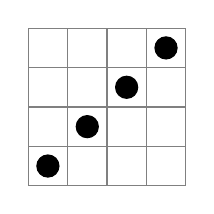
\begin{tikzpicture}[scale=0.5]
        \draw[gray] (0,0) grid (4,4);
        \filldraw[black] (0.5,0.5) circle (8pt);
        \filldraw[black] (1.5,1.5) circle (8pt);
        \filldraw[black] (2.5,2.5) circle (8pt);
        \filldraw[black] (3.5,3.5) circle (8pt);
      \end{tikzpicture}
      \caption{1234}
    \end{subfigure}
    \begin{subfigure}[b]{0.3\textwidth}
      \centering
      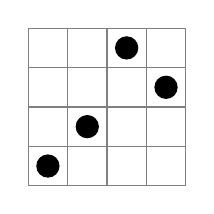
\begin{tikzpicture}[scale=0.5]
        \draw[gray] (0,0) grid (4,4);
        \filldraw[black] (0.5,0.5) circle (8pt);
        \filldraw[black] (1.5,1.5) circle (8pt);
        \filldraw[black] (2.5,3.5) circle (8pt);
        \filldraw[black] (3.5,2.5) circle (8pt);
      \end{tikzpicture}
      \caption{1243}
    \end{subfigure}
    \begin{subfigure}[b]{0.3\textwidth}
      \centering
      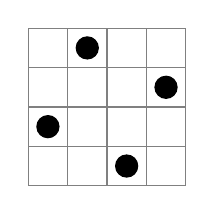
\begin{tikzpicture}[scale=0.5]
        \draw[gray] (0,0) grid (4,4);
        \filldraw[black] (0.5,1.5) circle (8pt);
        \filldraw[black] (1.5,3.5) circle (8pt);
        \filldraw[black] (2.5,0.5) circle (8pt);
        \filldraw[black] (3.5,2.5) circle (8pt);
      \end{tikzpicture}
      \caption{2413}
    \end{subfigure}

  \end{center}
  \caption{Pictorial representations of selected permutations.}
  \label{fig:im2413}
\end{figure}
    
\subsection{Special permutations}

An \emph{interval} refers to a set of integers appearing contiguously in a permutation, e.g. $3645$ is an interval in $213645$. A permutation $\pi$ is \emph{simple} if it does not contain any non-trivial intervals. For instance, $2413$ is simple while $1243$ is not (both $12$ and $43$ are intervals). We call $\pi$ an \emph{inflation} of $\sigma$ if it can be obtained from $\sigma$ by substituting points of $\sigma$ for permutations. We denote $\pi$ as an inflation of $\sigma$ by $\pi = \sigma[\alpha_1,\ldots,\alpha_{|\sigma|}]$, where $\alpha_1,\ldots,\alpha_{|\sigma|}$ are permutations that inflate $\sigma$ into $\pi$. Consider the example of $1243$ as an inflation of $12$, so $1243 = 12[12,21]$. In this case, it is also an inflation of $12$ by $1$ and $132$ as in $1243=12[1,132]$. There is a fundamental result by Albert and Atkinson~\cite{albertatkinsonrestricted} which says that if $\sigma$ is of length at least three and simple, then for any $\pi$ which is an inflation of $\sigma$ there is always a unique way to inflate $\sigma$ into $\pi$. Hence, $12$ and $21$ are special. 

A \emph{decreasing (increasing) permutation} of length $k$ is $k\ldots321$, respectively $123\ldots k$. A permutation $\pi$ is \emph{layered}, if it is an increasing sequence of decreasing permutations. To be exact, a layered permutation $\pi$ is a concatenation of smaller permutations $\pi= \pi_1\pi_2\ldots\pi_\ell$ such that for all $1 \leq i \leq \ell$, $\pi_i$ is a decreasing sequence of consecutive integers satisfying the following: if $x \in \pi_i$ and $y \in \pi_j$ with $i<j$, then $x<y$. For instance, 321465987 can be partitioned as $321|4|65|987$, so it is layered. On the other hand, 2413 is not layered. This brings us to the notion of sum and skew-sum of permutations. Let $\pi_1$ and $\pi_2$ be permutations of lengths $k$ and $\ell$. We say that $\pi$ is a \emph{sum of $\pi_1$ and $\pi_2$}, denoted by $\pi = \pi_1\oplus\pi_2$, if $\pi$ consists of two intervals $\pi[1]\cdots\pi[k]$ and $\pi[k+1]\cdots\pi[\ell]$ such that $\pi[1]\cdots\pi[k]$ is order-isomorphic to $\pi_1$, $\pi[k+1]\cdots\pi[\ell]$ is order-isomorphic to $\pi_2$, and $\pi[i] < \pi[j]$ for all $i\leq k$ and $j>k$. Similarly, $\pi$ is a \emph{skew-sum of $\pi_1$ and $\pi_2$}, denoted by $\pi = \pi_1\ominus \pi_2$, if $\pi$ consists of the two intervals as above, except this time we require that $\pi[i] > \pi[j]$ for all $i\leq k$ and $j > k$. A permutation is called \emph{sum-indecomposable} if it cannot be expressed as a sum of two non-empty permutations. Analogously, \emph{skew-indecomposable} permutations cannot be expressed as skew sums of non-empty permutations. With this new notation in place, a layered permuation with $k$ layers is $\pi = \pi_1\oplus\cdots\oplus \pi_k$ such that all $\pi_i$ are decreasing permutations. A permutation is called \emph{separable}, if it can be obtained from single points by repeated application of sum and skew-sum. For instance, $42315=(1\ominus (1\oplus 1)\ominus 1)\oplus 1$ is separable, but $2413$ is not.

\subsection{Permutation classes}
A \emph{permutation class} $\C$ is a set of permutations which is closed under taking subpermutations, i.e. if $\pi$ is in $\C$ and $\sigma \subseteq \pi$, then $\sigma$ is also in $\C$. Given that the subpermutation relation is a partial order on a permutation class $\C$, there is a minimal set of forbidden permutations called the \emph{basis} $\B$ of $\C$. We also write $\C = \Av(\B)$ to make explicit the fact that $\C$ is the set of avoiders of $\B$. For example, the class $\Av(231,312)$ is the class of layered permutations. Similarly, $\Av(2413, 3142)$ is the class of separable permutations. The subset of a class $\C$ containing only permutations of length $n$ is referred to by $\C_n$. Hence, $\C = \bigcup_{n\geq0}\C_n$. We use $|\C_n|$ to denote the number of elements of length $n$ in $\C$. 

To enumerate a permutation class $\C$ means to provide a sequence $(a_n)_{n\geq 0}$ such that $a_n = |\C_n|$. Given that $(a_n)_n$ has infinitely many terms, we need a clever data structure to store it in finite memory. A \emph{generating function} $C(z)$ of $\C$ is a formal power series $C(z) = \sum_{n\geq 0}a_nz^n$ with the coefficient of $z^n$ being the $n$-th term of the sequence. Ideally we would know the closed form of $C(z)$, e.g. the closed form of $C(z) = \sum_{n\geq 0}z^n = 1/(1-z)$. A rational generating function is one whose closed form is a ratio of two polynomials. An algebraic generating function $f = f(z)$ is a root of a polynomial equation in $f$ and $z$. As a shortcut, when we say that a generating function enumerating $\C$ is rational/algebraic/etc., we mean that the closed form of the formal power series storing the counting sequence which enumerates $\C$ is rational/algebraic/etc.

All work in this thesis is on enumeration of permutation (grid) classes. Whenever we obtain a generating function and a counting sequence, we refer to the result as an ``exact enumeration''. On the other hand, if we can only comment on the quality of the generating function yet we did not find one explicitly, we do not use the term ``exact''. This constitutes a slight deviation from the customary usage of the term ``exact enumeration''. We do not use ``exact'' to create contrast against ``asymptotic''. Mentioning it here hopefully prevents confusion later on.


It may not always be possible to find the generating function for a class. One cruder way of ``enumerating'' a permutation class is \emph{asymptotically}, by determining its growth rate. The \emph{growth rate} of a class $\C$ is denoted by $\gr{\C}$ and is defined as below provided that the limit exists.
$$\gr{\C} = \lim_{n\to\infty}\sqrt[n]{|\C_n|}$$
Naturally, if the above limit does not exist despite being conjectured to always exist, we speak about an \emph{upper growth rate} of $\C$ defined as $\lim\sup_{n\to\infty}\sqrt[n]{|\C_n|}$ and a \emph{lower growth rate} of $\C$ defined as $\lim\inf_{n\to\infty}\sqrt[n]{|\C_n|}$. Conveniently, by proving F\"{u}redi-Hajnal conjecture, Marcus and Tardos~\cite{marcus04growthrate} also proved Stanley-Wilf conjecture that the upper growth rate is finite for all proper permutation classes. Together with Arratia's observation in~\cite{arratia1999}, this implies that all permutation classes with basis of size one --- also called \emph{principal} classes --- have finite growth rates. Interestingly, there were conjectures about the growth rates of principal classes and all were refuted by this point in time. First Arratia~\cite{arratia1999} conjectured that for every permutation $\sigma$, $\gr{\Av(\sigma)} \leq (k-1)^2$. However, in 2006 Albert, Elder, Rechnitzer, Westcott, and Zabrocki~\cite{albert2006wilf} disproved this by showing that $\gr{\Av(1324)} > 9.47 > (4-1)^2$. B\'ona first suggested in~\cite{bona2005wilf} that layered permutations may be the easiest to avoid, i.e. their principal avoider classes tend to have highest growth rates, an impression strengthened by the result of Albert et al.~\cite{albert2006wilf}. However, in 2013 Fox~\cite{fox2013wilf} confirmed what we knew already: that we do not understand the growth rates of permutation classes very well. His result states that almost all patterns $\sigma$ of length $k$ have growth rates of a completely different order than we thought: $\gr{\Av(\sigma)} = 2^{\Omega(k)}$. Although this was tangential to the core topic of the thesis, it shows that permutation patterns form an exciting area to study.
